\subsection{General Overview}

Each team can choose an arbitrary payload to design and build. The team decided to develop long-term a set of gliders that are, once deployed from the rocket, flying back to the ground in formation. 


For this year, the team prepared a technology demonstrator consisting of only one glider deployed at apogee. This can be extrapolated for a fleet of 7 gliders. The challenge of building more gliders lies in fitting them into a constrained space in the rocket. 

\paragraph{Motivation for choosing the payload}
\hfill \break
Rovers such as Curiosity or Spirit have studied Martian terrain and sent back scientific data which may answer questions regarding the origin of life. However, in-situ atmospheric measurements of Mars on longer distances are missing. In order to solve this need, gliders, balloons, or powered planes should overfly Mars and land in areas where rovers cannot. Several projects are proposed by NASA in these directions such as the Preliminary Research Aerodynamic Design to Land on Mars (Prandtl-m) Airplane which aims to be released from a 3U CubeSat and do a 1-hour descent onto the surface of Mars.

Inspired by the Prandtl-m project, our team aimed to design and build an autonomous glider for the Spaceport America Cup competition, and learn more about the flight dynamics and control of such a complex system.

% ref
% @misc{mars,
%   title = {Could This Become the First Mars Airplane?},
%   howpublished = {\url{https://www.nasa.gov/centers/armstrong/features/mars_airplane.html}},
%   note = {Accessed: 2016-07-06}
% }

\begin{table}[h!]
\centering
\begin{tabular}{|p{0.9\columnwidth}|}
\hline
    The payload shall weight 8.8 lb (3.9 kg). \\ \hline
    The payload shall consist of a glider and ballast.  \\ \hline
    The glider shall be deployed at apogee. \\ \hline
    The glider shall deploy its wings passively once ejected from the rocket. \\ \hline
    The glider shall be equipped with an RTK (Real Time Kinematic) GPS used for navigation. \\ \hline
    The glider shall be equipped with a Commercial-Off-The-Shelve autopilot and a pitot tube \\ \hline
    The glider's battery life shall be 1.5 hours. \\ \hline
\end{tabular}
\caption{Top Level Requirements for the payload}
\label{table:se_topLevelR}
\end{table}


\subsection{Design and Manufacturing of one glider}
%Pictures from report here

Due to space constraints, the glider was chosen to be a flying wing with the wings folded in front. XFLR simulations experiments with different airfoils, wing span, wing sweep were performed until the acceptable flight parameters were obtained. The final airfoil is a MH45, with improved (3\%) reflex.

The plane parameters are presented in Table \ref{plane_param}.

\begin{table}[h!]
\centering
\begin{tabular}{|l|l|l|}
\hline
\textbf{wing span}      & 0.72 {[}m{]}        & 2.36 {[}ft{]}        \\ \hline
\textbf{wing area}      & 0.07 {[}m$^2${]}    & 0.75 {[}ft $^2${]}   \\ \hline
\textbf{mass}           & 0.27 {[}kg{]}       & 0.61 {[}lb{]}        \\ \hline
\textbf{wing load}      & 4.06 {[}kg/m$^2${]} & 0.83 {[}lb/ft$^2${]} \\ \hline
\textbf{root chord}     & 0.11 {[}m{]}        & 0.36 {[}in{]}        \\ \hline
\textbf{neutral point}  & 0.09 {[}m{]}        & 0.29 {[}in{]}        \\ \hline
\textbf{tip twist}      & -4$^\circ$        &                      \\ \hline
\textbf{aspect ratio}   & 7.50                &                      \\ \hline
\textbf{root-tip chord} & 21$^\circ$        &                      \\ \hline
\end{tabular}
\caption{Plane parameters}
\label{plane_param}
\end{table}


The optimal flight data is presented in Table \ref{flight_param}.

\begin{table}[h!]
\centering
\begin{tabular}{|l|l|}
\hline
\textbf{speed}                    & 18.42 {[}m/s{]} \\ \hline
\textbf{angle-of-attack}          & 4.5$^\circ$                        \\ \hline
\textbf{lift coefficient ($C_L$)} & 0.21                               \\ \hline
\textbf{drag coefficient ($C_D$)} & 0.02                               \\ \hline
\textbf{$C_L$/$C_D$}              & 10                                 \\ \hline
\end{tabular}
\caption{Flight parameters}
\label{flight_param}
\end{table}


The glider was designed in Solidworks. All the components of the glider are encapsulated either in the fuselage, or in the wings, as it can be seen in Figure \ref{f:fuseg} and Figure  \ref{f:wings}.


\begin{figure}[h!]
    \centering
        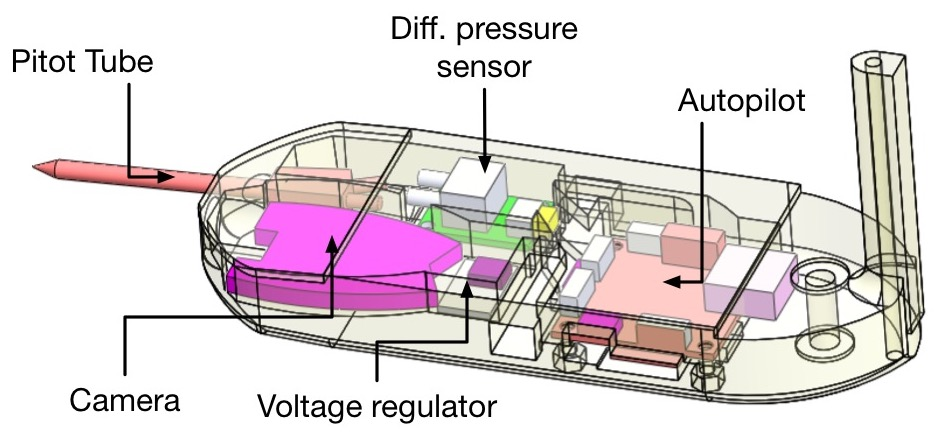
\includegraphics[width=0.5\textwidth]{img/fuselage.jpg}
        \caption{Fuselage with components encapsulated}
        \label{f:fuseg}
 \end{figure}

\begin{figure}[h!]
    \centering
        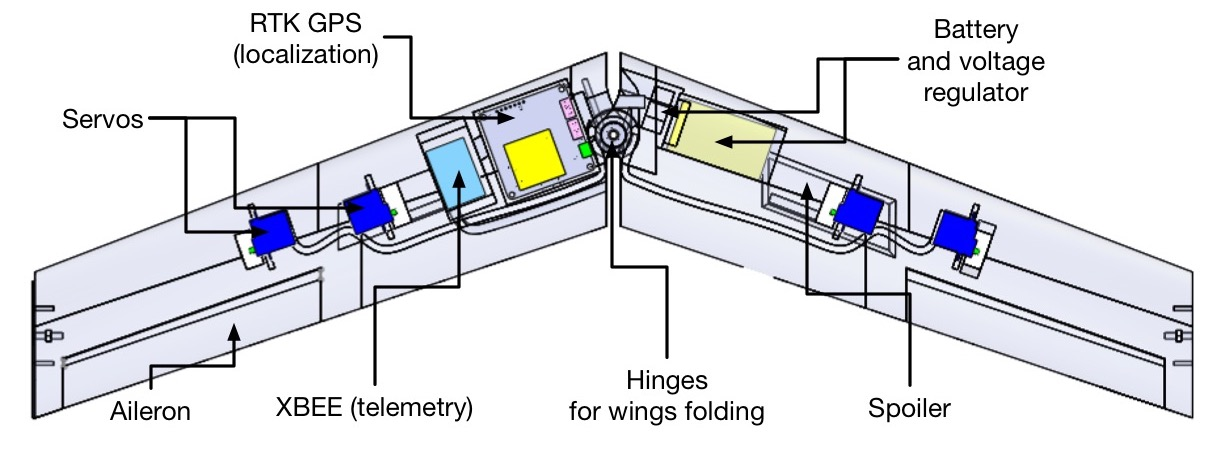
\includegraphics[width=0.5\textwidth]{img/wings.jpg}
        \caption{Wings with components encapsulated}
        \label{f:wings}
 \end{figure}


The wings are folded in front, as it can be seen in Figure \ref{f:folding}.

\begin{figure}[h!]
    \centering
        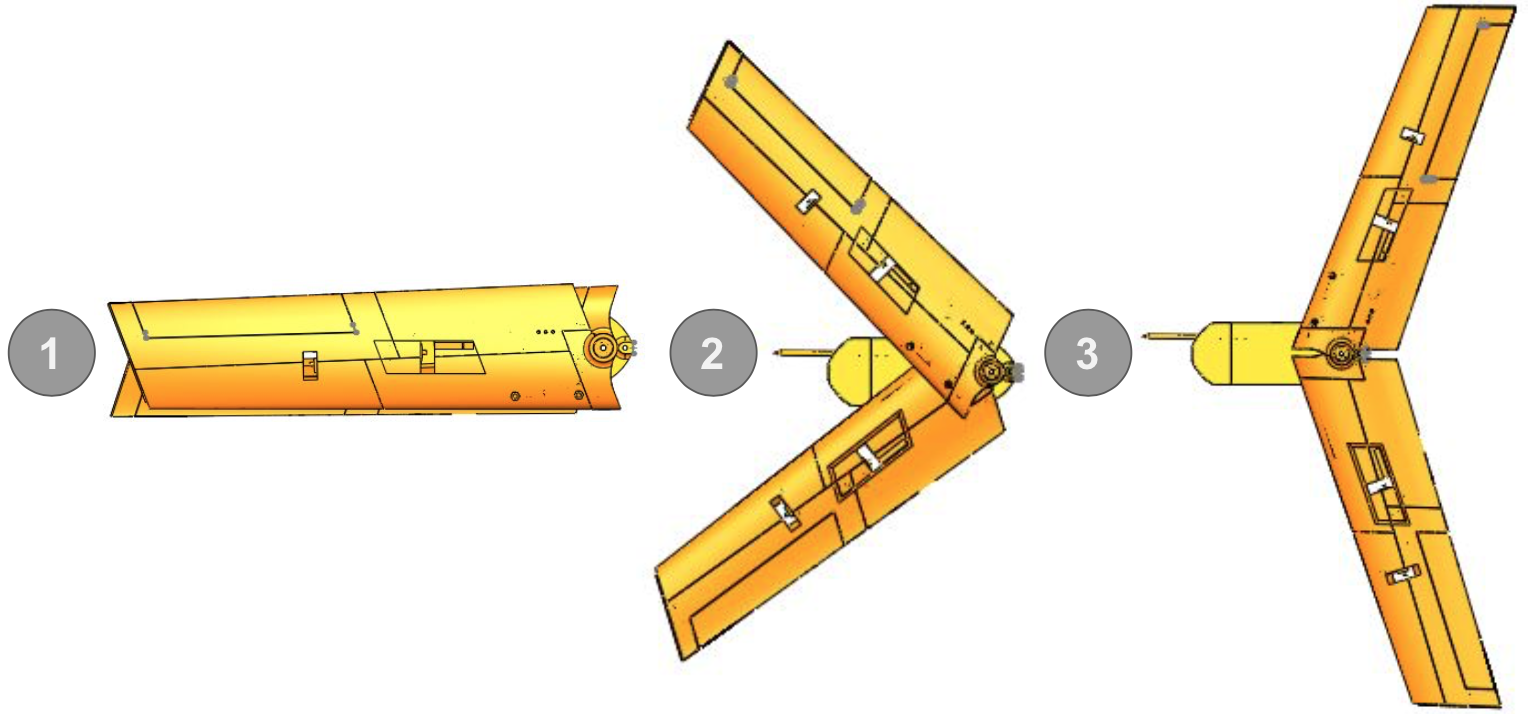
\includegraphics[width=0.5\textwidth]{img/folding.png}
        \caption{Unfolding steps 1. The glider is fully folded in its bay. 2. The glider is ejected from the rocket and starts unfolding. 3. The glider is unfolded and starts flying back to the ground}
        \label{f:folding}
 \end{figure}

\subsection{Navigation and Control of the fleet of gliders}
\label{subsection:navcontrol}
%Ultrawide beacons 
%Formation
%Check for alternative options, instead of GPS

